% ============================================================================
%  The Himbaechel Architecture
%  How nextpnr scales place-and-route to Xilinx 7-series (and beyond)
%
%  Based on the verified analysis in ../xilinx-porting/01-himbaechel-architecture.md
%  and ../xilinx-porting/03-algorithmic-diff.md (nextpnr @ nextpnr-0.11.1, 62e659e).
%  All code listings are excerpts from the real source tree.
%  Build: lualatex himbaechel.tex  (x2 for TOC)
% ============================================================================
\documentclass[11pt,a4paper]{article}

% ---------------------------------------------------------------- packages
\usepackage[default]{sourcesanspro}      % body font: Source Sans Pro
\usepackage{sourcecodepro}               % code font: Source Code Pro
\renewcommand{\familydefault}{\sfdefault}
\usepackage[T1]{fontenc}
\usepackage{microtype}
\usepackage{geometry}
\geometry{margin=2.4cm,top=2.6cm,bottom=2.8cm,headheight=14pt}

\usepackage{xcolor}
\usepackage{tikz}
\usetikzlibrary{arrows.meta,positioning,fit,backgrounds,calc,shadows.blur,
                shapes.geometric,decorations.pathreplacing}

\usepackage{tcolorbox}
\tcbuselibrary{listings,skins,breakable,hooks}

\usepackage{listings}
\usepackage{booktabs}
\usepackage{array}
\usepackage{multicol}
\usepackage{tabularx}
\usepackage{fancyhdr}
\usepackage{titlesec}
\usepackage[colorlinks=true,linkcolor=accent1,urlcolor=accent2,
            citecolor=accent1]{hyperref}
\usepackage{enumitem}
\setlist{topsep=2pt,itemsep=2pt,parsep=0pt}
\emergencystretch=2.2em

% ---------------------------------------------------------------- palette
\definecolor{primary}{RGB}{40,44,88}      % deep navy
\definecolor{accent1}{RGB}{0,110,180}     % blue
\definecolor{accent2}{RGB}{0,150,110}     % green
\definecolor{accent3}{RGB}{220,95,30}     % orange
\definecolor{warn}{RGB}{190,30,45}        % red
\definecolor{bg}{RGB}{246,247,250}        % light panel
\definecolor{codebg}{RGB}{250,251,253}
\definecolor{grayline}{RGB}{120,125,140}

% ---------------------------------------------------------------- headings
\titleformat{\section}
  {\sffamily\Large\bfseries\color{primary}}
  {\thesection}{0.7em}{}
  [{\vspace{0.1ex}\color{accent1}\titlerule[2pt]\vspace{0.2ex}}]
\titleformat{\subsection}
  {\sffamily\large\bfseries\color{accent1}}
  {\thesubsection}{0.6em}{}
\titleformat{\subsubsection}
  {\sffamily\normalsize\bfseries\color{primary}}
  {\thesubsubsection}{0.6em}{}

% ---------------------------------------------------------------- headers
\pagestyle{fancy}
\fancyhf{}
\fancyhead[L]{\sffamily\footnotesize\color{grayline}THE HIMBAECHEL ARCHITECTURE}
\fancyhead[R]{\sffamily\footnotesize\color{grayline}\thepage}
\renewcommand{\headrulewidth}{0.4pt}
\renewcommand{\headrule}{\color{accent1}\hrule width\headwidth height 0.4pt}

% ---------------------------------------------------------------- listings
\lstdefinestyle{cppstyle}{
  language=C++,
  basicstyle=\ttfamily\fontsize{8.2pt}{10pt}\selectfont,
  keywordstyle=\bfseries\color{accent1},
  commentstyle=\itshape\color{grayline},
  stringstyle=\color{accent3},
  numbers=left,
  numberstyle=\tiny\color{grayline},
  numbersep=6pt,
  tabsize=4,
  showstringspaces=false,
  breaklines=true,
  breakatwhitespace=true,
  columns=fullflexible,
  keepspaces=true,
  literate={ä}{{\"a}}1 {ö}{{\"o}}1 {ü}{{\"u}}1 {ß}{{\ss}}1,
  aboveskip=0pt, belowskip=0pt,
  xleftmargin=8pt,
}
\lstdefinestyle{pystyle}{
  language=Python,
  basicstyle=\ttfamily\fontsize{8.2pt}{10pt}\selectfont,
  keywordstyle=\bfseries\color{accent1},
  commentstyle=\itshape\color{grayline},
  stringstyle=\color{accent3},
  numbers=left, numberstyle=\tiny\color{grayline}, numbersep=6pt,
  tabsize=4, showstringspaces=false, breaklines=true,
  columns=fullflexible, keepspaces=true,
  aboveskip=0pt, belowskip=0pt, xleftmargin=8pt,
}
\lstdefinestyle{bashstyle}{
  language=bash,
  basicstyle=\ttfamily\fontsize{8.2pt}{10pt}\selectfont,
  keywordstyle=\bfseries\color{accent2},
  commentstyle=\itshape\color{grayline},
  stringstyle=\color{accent3},
  numbers=none, tabsize=4, showstringspaces=false, breaklines=true,
  columns=fullflexible, keepspaces=true,
  aboveskip=0pt, belowskip=0pt,
}

\newtcolorbox{cppfile}[1]{%
  enhanced, breakable,
  title={\ttfamily\footnotesize\detokenize{#1}},
  colback=codebg, colframe=accent1!60!white,
  boxrule=0.6pt, arc=2pt, left=0pt, right=0pt, top=4.5mm, bottom=0.5pt,
  attach boxed title to top left={yshift=-2.6mm,xshift=3mm},
  boxed title style={colback=accent1,colframe=accent1,arc=1.5pt,
                     boxrule=0pt,left=2pt,right=2pt,top=1pt,bottom=1pt},
  before upper={\vspace{-2pt}},
}

% ---------------------------------------------------------------- callouts
\newtcolorbox{factbox}[1]{%
  enhanced, breakable, colback=accent2!8, colframe=accent2,
  boxrule=0.7pt, arc=2.5pt, left=6pt, right=6pt, top=4mm, bottom=4pt,
  title={\sffamily\footnotesize\bfseries #1},
  attach boxed title to top left={yshift=-2.4mm,xshift=3mm},
  boxed title style={colback=accent2,colframe=accent2,arc=1.5pt,
                     boxrule=0pt,left=2pt,right=2pt,top=1pt,bottom=1pt},
}
\newtcolorbox{warnbox}[1]{%
  enhanced, breakable, colback=warn!7, colframe=warn,
  boxrule=0.7pt, arc=2.5pt, left=6pt, right=6pt, top=4mm, bottom=4pt,
  title={\sffamily\footnotesize\bfseries #1},
  attach boxed title to top left={yshift=-2.4mm,xshift=3mm},
  boxed title style={colback=warn,colframe=warn,arc=1.5pt,
                     boxrule=0pt,left=2pt,right=2pt,top=1pt,bottom=1pt},
}

% tikz helpers
\tikzset{
  flowbox/.style={rectangle, rounded corners=1.5mm, draw=primary, thick,
                  fill=white, align=center, font=\sffamily\small,
                  inner sep=4pt, minimum height=9mm,
                  drop shadow={shadow xshift=0.6mm,shadow yshift=-0.6mm,opacity=0.15}},
  flowboxaccent/.style={flowbox, draw=accent1, fill=accent1!5},
  flowboxgreen/.style={flowbox, draw=accent2, fill=accent2!6},
  flowboxwarm/.style={flowbox, draw=accent3, fill=accent3!6},
  flowboxgray/.style={flowbox, draw=grayline, fill=bg},
  arr/.style={-{Stealth[length=2.6mm]}, thick, color=accent1},
  arrdark/.style={-{Stealth[length=2.6mm]}, thick, color=primary},
  lbl/.style={font=\sffamily\footnotesize\itshape\color{grayline},
              inner sep=1pt, fill=white},
}

% ---------------------------------------------------------------- title
\title{\vspace{-14mm}
  {\sffamily\bfseries\color{primary}\fontsize{26pt}{30pt}\selectfont
   The Himbaechel Architecture}\\[4mm]
  {\sffamily\large\color{accent1}
   How nextpnr scales place-and-route to Xilinx 7-series}\\[1.5mm]
  {\sffamily\normalsize\color{grayline}
   An illustrated guide to the chip database, the uarch plugin API, and the\\
   xc7 implementation in \texttt{himbaechel/uarch/xilinx}}}
\author{\sffamily\small nextpnr documentation working group}
\date{\sffamily\small \today \quad$\cdot$\quad nextpnr \texttt{nextpnr-0.11.1} (\texttt{62e659e})}

\begin{document}

% ===========================================================================
%  TITLE PAGE
% ===========================================================================
\begin{titlepage}
\maketitle
\vspace{1mm}
\begin{center}
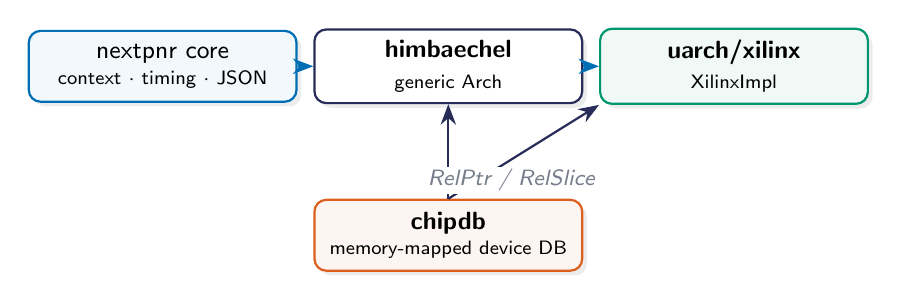
\begin{tikzpicture}[scale=1]
  \node[flowboxaccent, minimum width=34mm] (fw) {nextpnr core\\[-0.6mm] {\scriptsize context $\cdot$ timing $\cdot$ JSON}};
  \node[flowbox, minimum width=34mm, right=2mm of fw] (arch) {\textbf{himbaechel}\\{\scriptsize generic Arch}};
  \node[flowboxgreen, minimum width=34mm, right=2mm of arch] (uarch) {\textbf{uarch/xilinx}\\{\scriptsize XilinxImpl}};
  \node[flowboxwarm, minimum width=34mm, below=12mm of arch] (chipdb) {\textbf{chipdb}\\[-0.6mm] {\scriptsize memory-mapped device DB}};
  \draw[arr] (fw) -- (arch);
  \draw[arr] (arch) -- (uarch);
  \draw[arrdark] (chipdb.north) -- (arch.south);
  \draw[arrdark] (chipdb.north) -- (uarch.south west);
  \node[lbl, above=0.5mm of chipdb, xshift=8mm] {RelPtr / RelSlice};
\end{tikzpicture}
\end{center}
\vfill
\begin{tcolorbox}[enhanced, colback=bg, colframe=primary!30, arc=2mm,
                   title={\sffamily\footnotesize\bfseries About this document}]
\sffamily\small
This guide explains \emph{how himbaechel works} from the inside: the
deduplicated chip database and its relative-pointer model, the uarch
plugin interface, and how the Xilinx 7-series uarch implements packing,
placement, routing, timing, and FASM bitstream generation on top of it.
It is written for engineers who already know what place-and-route does
and want to understand this specific implementation well enough to
modify it. Code excerpts are taken verbatim from the source tree at tag
\texttt{nextpnr-0.11.1}; line numbers refer to that checkout.
\end{tcolorbox}
\end{titlepage}

\tableofcontents
\clearpage

% ===========================================================================
\section{Motivation: why himbaechel exists}

nextpnr has two generations of architecture interfaces. The original
one---colloquially ``Viaduct''---builds a \emph{flat, in-memory routing
graph} at startup: every wire, pip, and bel is instantiated as a C++
object and linked together. That is fine for small devices (iCE40,
ECP5, Gowin) but the object overhead explodes past roughly 20{,}000
logic elements. A Xilinx Artix-7 die has tens of thousands of slices,
each with many pips and wires; a flat model would cost multiple
gigabytes of RAM.

\textbf{Himbaechel} (the nextpnr maintainers' name for the ``bigger
arches'' framework, documented upstream in \texttt{docs/himbaechel.md})
solves this by moving the device model out of C++ objects and into a
\emph{compile-time generated, deduplicated binary database}---the
\emph{chipdb}---which is memory-mapped at runtime and read through
\emph{relative pointers}. Million-LUT devices then fit in roughly
100\,MB instead of multi-GB, and most of the routing-graph queries
become flat array lookups into POD (plain-old-data) structures.

\begin{factbox}{Scaling in one sentence}
Viaduct stores the device as a heap of interlinked C++ objects; himbaechel
stores it as a position-independent binary blob of deduplicated PODs that
is mapped into memory and traversed with relative pointers. The
place-and-route \emph{algorithms} stay shared; only the device model
changes.
\end{factbox}

The framework supports multiple device families by delegating to
per-family ``micro-architectures'' (uarchs): \texttt{example},
\texttt{gowin}, \texttt{gatemate}, \texttt{ng-ultra}, and---the subject
of this guide---\texttt{xilinx} for Xilinx 7-series (xc7).

% ===========================================================================
\section{Architecture at a glance}

\begin{figure}[htbp]
\centering
\resizebox{\textwidth}{!}{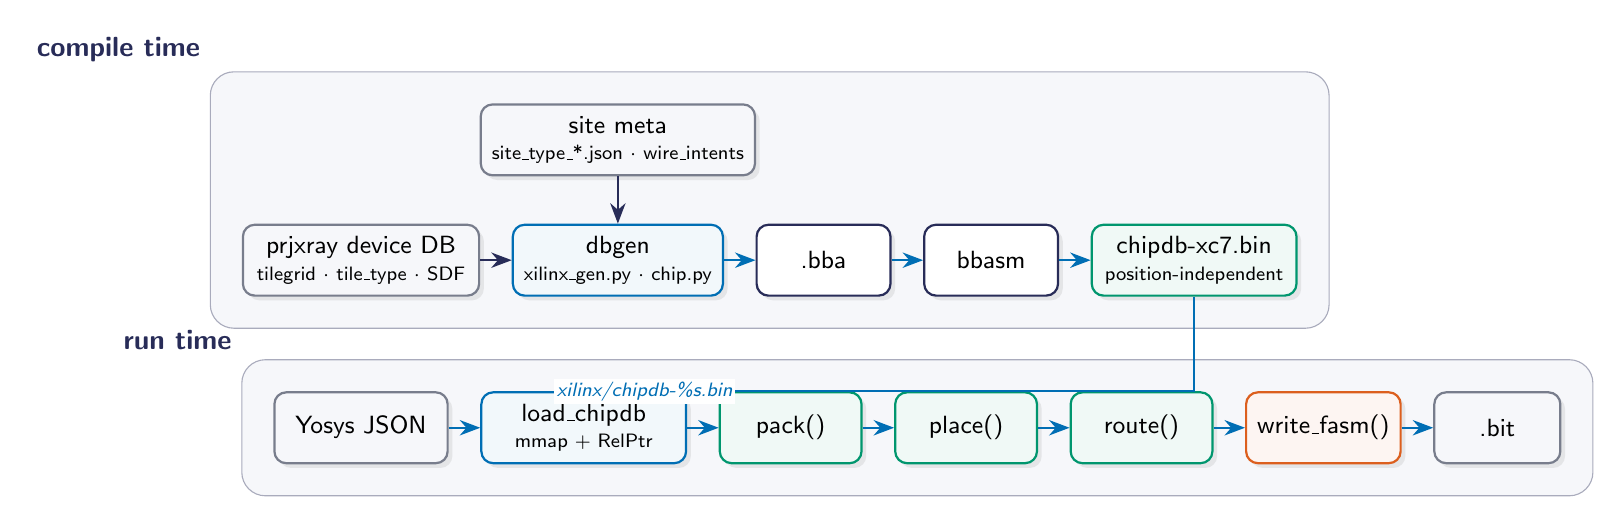
\begin{tikzpicture}[node distance=3.5mm and 4mm]
  % ---- compile-time row ----
  \node[flowboxgray, minimum width=30mm] (prjxray) {prjxray device DB\\[-0.5mm]{\scriptsize tilegrid $\cdot$ tile\_type $\cdot$ SDF}};
  \node[flowboxaccent, minimum width=26mm, right=of prjxray] (gen) {dbgen\\[-0.5mm]{\scriptsize xilinx\_gen.py $\cdot$ chip.py}};
  \node[flowbox, minimum width=17mm, right=of gen] (bba) {.bba};
  \node[flowbox, minimum width=17mm, right=of bba] (bbasm) {bbasm};
  \node[flowboxgreen, minimum width=26mm, right=of bbasm] (bin) {chipdb-xc7.bin\\[-0.5mm]{\scriptsize position-independent}};
  \node[flowboxgray, minimum width=26mm, above=6mm of gen] (meta) {site meta\\[-0.5mm]{\scriptsize site\_type\_*.json $\cdot$ wire\_intents}};
  \draw[arrdark] (prjxray.east) -- (gen.west);
  \draw[arrdark] (meta.south) -- (gen.north);
  \draw[arr] (gen.east) -- (bba.west);
  \draw[arr] (bba.east) -- (bbasm.west);
  \draw[arr] (bbasm.east) -- (bin.west);

  % ---- run-time row ----
  \node[flowboxgray, minimum width=22mm, below=12mm of prjxray] (json) {Yosys JSON};
  \node[flowboxaccent, minimum width=26mm, right=of json] (load) {load\_chipdb\\[-0.5mm]{\scriptsize mmap + RelPtr}};
  \node[flowboxgreen, minimum width=18mm, right=of load] (pack) {pack()};
  \node[flowboxgreen, minimum width=18mm, right=of pack] (place) {place()};
  \node[flowboxgreen, minimum width=18mm, right=of place] (route) {route()};
  \node[flowboxwarm, minimum width=18mm, right=of route] (fasm) {write\_fasm()};
  \node[flowboxgray, minimum width=16mm, right=of fasm] (bit) {.bit};

  \draw[arr] (bin.south) |- (load.north) node[lbl,pos=0.95,xshift=0mm] {\scriptsize xilinx/chipdb-\%s.bin};
  \draw[arr] (json.east) -- (load.west);
  \draw[arr] (load.east) -- (pack.west);
  \draw[arr] (pack.east) -- (place.west);
  \draw[arr] (place.east) -- (route.west);
  \draw[arr] (route.east) -- (fasm.west);
  \draw[arr] (fasm.east) -- (bit.west);

  \begin{scope}[on background layer]
    \node[fit=(prjxray)(meta)(gen)(bba)(bbasm)(bin), rounded corners=3mm,
          draw=primary!40, fill=bg, inner sep=4mm,
          label={[font=\sffamily\bfseries\color{primary}]north west:compile time}]{};
    \node[fit=(json)(load)(pack)(place)(route)(fasm)(bit), rounded corners=3mm,
          draw=primary!40, fill=bg, inner sep=4mm,
          label={[font=\sffamily\bfseries\color{primary}]north west:run time}]{};
  \end{scope}
\end{tikzpicture}}
\caption{End-to-end data flow: a Python generator converts prjxray device data
plus site metadata into a binary chipdb at build time; at run time nextpnr
memory-maps the blob and runs the standard pack $\to$ place $\to$ route $\to$
FASM pipeline against it.}
\label{fig:overview}
\end{figure}

Figure~\ref{fig:overview} shows the whole system. The essential idea:
\emph{everything device-specific that can be precomputed is precomputed
offline and shipped as one immutable binary file}. The runtime code
queries that file; it never builds a routing graph object model.

Three code layers cooperate at run time:

\begin{itemize}
\item \textbf{The generic Arch} (\texttt{himbaechel/arch.h, arch.cc})---
  a concrete subclass of the shared \texttt{BaseArch<ArchRanges>} that
  implements every nextpnr architecture API (bel/wire/pip iteration,
  names, bounds, delays, drawing) as queries over the chipdb PODs.
\item \textbf{The uarch plugin} (one \texttt{HimbaechelAPI} subclass per
  family; for xc7: \texttt{XilinxImpl} in \texttt{uarch/xilinx/})---
  supplies all the \emph{family-specific knowledge}: packing,
  legality, placement configuration, clock routing, FASM emission.
\item \textbf{The shared algorithms} (\texttt{common/place},
  \texttt{common/route})---the analytical placer (HeAP), the ePlace-style
  static placer, the SA placer, router1 and router2---which are
  family-agnostic and talk to the uarch only through callbacks.
\end{itemize}

% ===========================================================================
\section{The chip database}

\subsection{Generation pipeline}

The chipdb is produced at \emph{build time}. The Xilinx generator lives
in \texttt{himbaechel/\allowbreak uarch/\allowbreak xilinx/\allowbreak gen/} and is driven by CMake
(\texttt{add\_bba\_produce\_command}\allowbreak{} +
\texttt{add\_bba\_compile\_command}):

\begin{cppfile}{himbaechel/uarch/xilinx/CMakeLists.txt:32}
  \lstinputlisting[style=cppstyle]{snippets/devices.cmake}
\end{cppfile}

For each enabled device, \texttt{xilinx\_gen.py} imports the prjxray
database (\texttt{tilegrid.json}, \texttt{tile\_type\_*.json},
\texttt{package\_pins.csv}, \texttt{tileconn.json}, SDF timings) plus
the site metadata from the \texttt{nextpnr-xilinx-meta} submodule, and
emits a text \texttt{.bba} file. \texttt{bbasm} (the BBA assembler)
compiles that into the final position-independent binary blob. The key
generation steps:

\begin{enumerate}
\item \textbf{Enumerate tile types} and deduplicate them---a design with
  hundreds of identical CLB tiles stores \emph{one} \texttt{TileTypePOD},
  not hundreds.
\item \textbf{Build the wire/node graph}: intra-tile wires stay local;
  cross-tile connectivity is expressed through \emph{nodes} that merge
  electrically-connected wires (see \S\ref{sec:model}).
\item \textbf{Record sites and bels} from prjxray site types, filtered
  and remapped by \texttt{filters.py} (e.g.\ every 6LUT becomes a
  \texttt{SLICE\_LUTX} bel).
\item \textbf{Import timing}: pip and node delays from prjxray
  \texttt{src\_to\_dst} data, cell arcs from SDF
  (\texttt{parse\_sdf.py}).
\item \textbf{Serialize} everything through relative pointers
  (\texttt{himbaechel\_dbgen/chip.py}) into \texttt{.bba}, then
  assemble to binary.
\end{enumerate}

\subsection{Relative pointers: RelPtr and RelSlice}

The blob is position-independent because all cross-references inside it
are \emph{relative}: a \texttt{RelPtr<T>} stores a signed offset from
its own address to the target, and \texttt{RelSlice<T>} stores an
offset plus a count. Dereferencing adds the offset to the pointer's own
location---so the whole file can be mapped at any address and still be
internally consistent.

\begin{figure}[htbp]
\centering
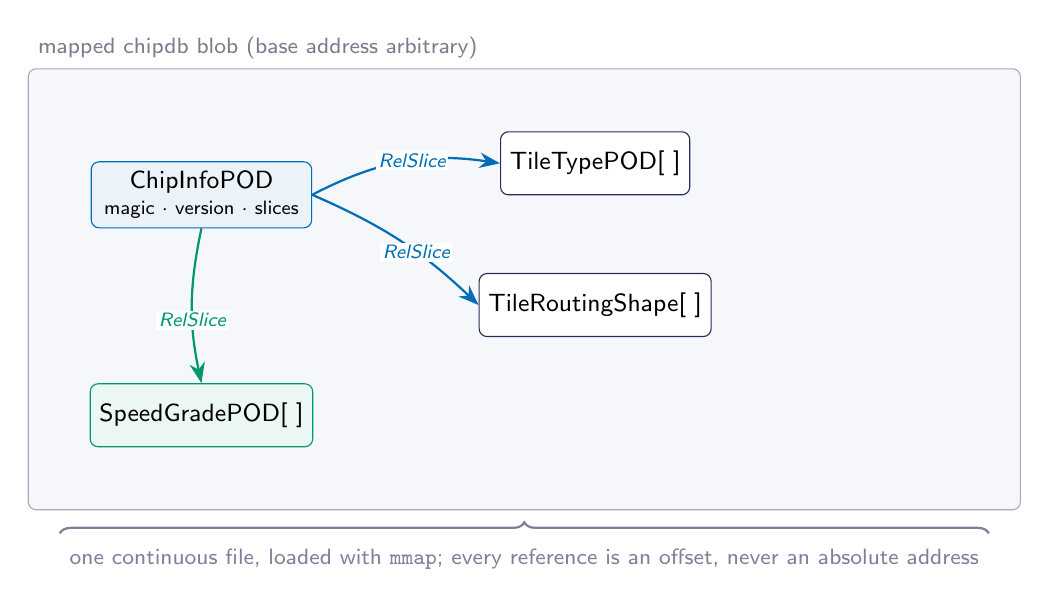
\begin{tikzpicture}[node distance=2mm and 3mm]
  \draw[fill=bg, draw=primary!40, rounded corners=1mm] (0,0) rectangle (12.6,-5.6);
  \node[font=\sffamily\footnotesize\color{grayline}, above right] at (0,0) {mapped chipdb blob (base address arbitrary)};
  % POD blocks
  \node[draw=accent1, fill=accent1!8, minimum width=28mm, minimum height=8mm,
        rounded corners=1mm, align=center, font=\sffamily\small] (c) at (2.2,-1.6) {ChipInfoPOD\\[-0.5mm]{\scriptsize magic $\cdot$ version $\cdot$ slices}};
  \node[draw=primary, fill=white, minimum width=22mm, minimum height=8mm,
        rounded corners=1mm, align=center, font=\sffamily\small] (tt) at (7.2,-1.2) {TileTypePOD[ ]};
  \node[draw=primary, fill=white, minimum width=22mm, minimum height=8mm,
        rounded corners=1mm, align=center, font=\sffamily\small] (ts) at (7.2,-3.0) {TileRoutingShape[ ]};
  \node[draw=accent2, fill=accent2!8, minimum width=22mm, minimum height=8mm,
        rounded corners=1mm, align=center, font=\sffamily\small] (sc) at (2.2,-4.4) {SpeedGradePOD[ ]};
  % relative pointer arcs
  \draw[arr, accent1, bend left=18] (c.east) to node[lbl,pos=0.55] {\scriptsize RelSlice} (tt.west);
  \draw[arr, accent1, bend left=10] (c.east) to node[lbl,pos=0.6] {\scriptsize RelSlice} (ts.west);
  \draw[arr, accent2, bend right=12] (c.south) to node[lbl,pos=0.6] {\scriptsize RelSlice} (sc.north);
  \draw[decorate, decoration={brace, amplitude=4pt}, thick, color=primary!60]
        (0.4,-5.9) -- (12.2,-5.9)
        node[midway, below=2pt, font=\sffamily\footnotesize\color{primary}]
             {one continuous file, loaded with \texttt{mmap}; every reference is an offset, never an absolute address};
\end{tikzpicture}
\caption{The chipdb is a single flat blob of POD arrays. The root
\texttt{ChipInfoPOD} is found at the file start; every other structure is
reached by relative offset from within the blob.}
\label{fig:relptr}
\end{figure}

The root structure is cast directly from the mapped memory:

\begin{cppfile}{himbaechel/chipdb.h:226}
  \lstinputlisting[style=cppstyle]{snippets/chipinfo_pod.h}
\end{cppfile}

\subsection{Loading and validating}

At startup the uarch asks the Arch to map its database:

\begin{cppfile}{himbaechel/arch.cc:117}
  \lstinputlisting[style=cppstyle]{snippets/load_chipdb.cc}
\end{cppfile}

Three consistency checks protect against mismatched binaries: the
\emph{magic number} \texttt{0x00ca7ca7} (``cat cat'', a himbaechel
signature), the \emph{database version} (6 in this checkout), and the
\emph{uarch name} stored in the blob. Extra constids (identifier
strings) that exist only in the device database are registered into
the \texttt{IdString} pool at the end---so the chipdb is also the
source of device-specific identifiers.

The default search path is \texttt{<share>/himbaechel/<path>}; the
Xilinx uarch requests \texttt{xilinx/chipdb-\%s.bin} with the die name
(\texttt{xilinx.cc:88}), and \texttt{xc7a35t} is aliased to the
\texttt{xc7a50t} die (\texttt{xilinx.cc:86-87}).

% ===========================================================================
\section{The device model: tiles, wires, pips, nodes}
\label{sec:model}

\subsection{Tile grid}

The device is a rectangular grid of \emph{tile instances}. Each
instance references a deduplicated \texttt{TileTypePOD} (which holds
the bels, wires, pips and groups common to all tiles of that type) and
a \texttt{TileRoutingShape\-POD} (which maps tile wires onto the global
\emph{node} graph). Tile names are synthesised as
\texttt{<prefix>X<X>Y\allowbreak<Y>}\allowbreak{} (\texttt{arch.cc:188-200}).

\begin{figure}[htbp]
\centering
\resizebox{\textwidth}{!}{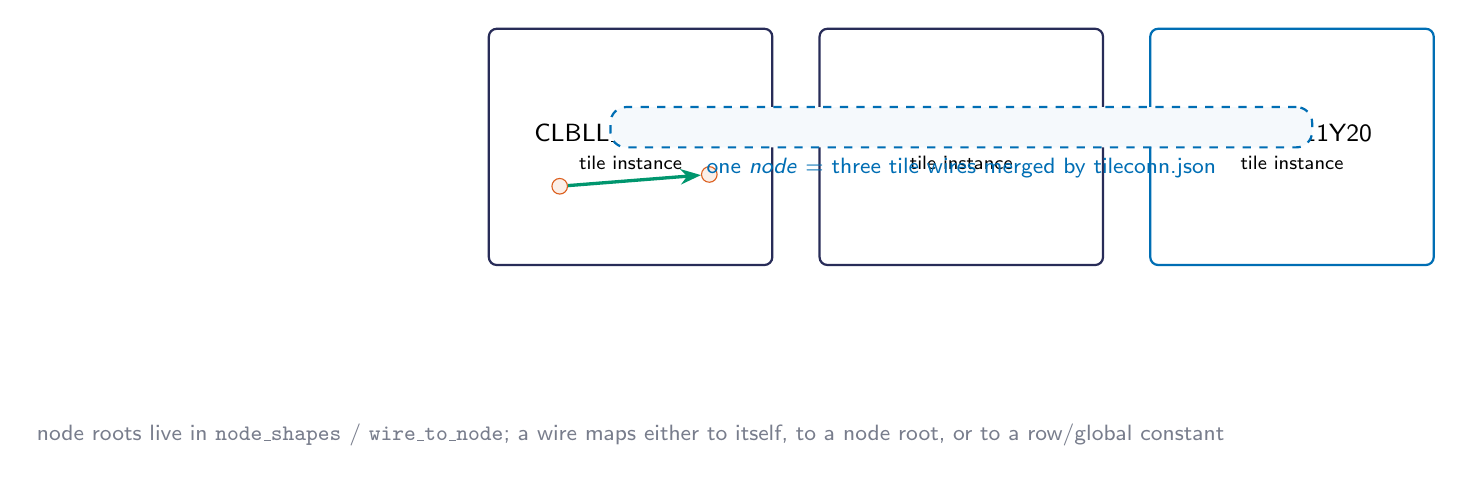
\begin{tikzpicture}
  % three tiles
  \foreach \x/\t/\c in {0/CLBLL\_L X10Y20/primary, 4.2/CLBLM\_R X11Y20/primary, 8.4/INT\_L X11Y20/accent1} {
    \node[draw=\c, thick, fill=white, minimum width=36mm, minimum height=30mm,
          rounded corners=1mm, align=center, font=\sffamily\small] (t\x) at (\x,0) {\t\\[-0.4mm]{\scriptsize tile instance}};
  }
  % wires inside tile 1
  \node[circle, draw=accent3, fill=accent3!10, inner sep=0.7mm] (w1) at (0.0,0.25) {};
  \node[circle, draw=accent3, fill=accent3!10, inner sep=0.7mm] (w2) at (1.0,-0.35) {};
  \node[circle, draw=accent3, fill=accent3!10, inner sep=0.7mm] (w3) at (-0.9,-0.5) {};
  % wires inside tile 2
  \node[circle, draw=accent3, fill=accent3!10, inner sep=0.7mm] (w4) at (4.2,0.25) {};
  % wires inside tile 3
  \node[circle, draw=accent3, fill=accent3!10, inner sep=0.7mm] (w5) at (8.4,0.25) {};
  % pip inside tile 1
  \draw[arr, accent2, very thick] (w3) -- (w2);
  % nodes: merged cross-tile wire groups
  \node[fit=(w1)(w4)(w5), draw=accent1, dashed, thick, rounded corners=2mm,
        fill=accent1!4, inner sep=1.5mm, label={[font=\sffamily\footnotesize,color=accent1]south:one \emph{node} = three tile wires merged by tileconn.json}]{};
  \node[font=\sffamily\footnotesize\color{grayline}, anchor=north] at (0,-3.4)
       {node roots live in \texttt{node\_shapes} / \texttt{wire\_to\_node}; a wire maps either to itself, to a node root, or to a row/global constant};
\end{tikzpicture}}
\caption{Wires are local to tiles; electrical connectivity across tile
boundaries is represented by \emph{nodes}. The router moves between tile
wires; \texttt{wire\_to\_node} tells it which wires are the same net.}
\label{fig:tiles}
\end{figure}

\subsection{Wire-to-node mapping}

Each tile wire carries a \texttt{RelNodeRefPOD} that classifies it:

\begin{cppfile}{himbaechel/chipdb.h:116}
  \lstinputlisting[style=cppstyle]{snippets/relnoderef.h}
\end{cppfile}

\begin{itemize}
\item \texttt{MODE\_TILE\_WIRE}---the wire is its own node (no merging);
\item \texttt{MODE\_IS\_ROOT}---this wire \emph{is} the root of a
  merged node (carries the timing/delay info);
\item \texttt{MODE\_ROW\_CONST} / \texttt{MODE\_GLB\_CONST}---the wire
  is part of a row- or globally-shared constant net (VCC/GND backbones).
\end{itemize}

Pips connect wires \emph{within} a tile (or via the site pips inside a
bel's site); they carry a timing index into the speed-grade data and an
opaque \texttt{extra\_data} pointer used by the family (the Xilinx
uarch stores \texttt{XlnxPipExtraDataPOD} there---e.g.\ LUT-permutation
pip configuration):

\begin{cppfile}{himbaechel/chipdb.h:74}
  \lstinputlisting[style=cppstyle]{snippets/pipdata.h}
\end{cppfile}

% ===========================================================================
\section{The uarch plugin API}

\begin{figure}[htbp]
\centering
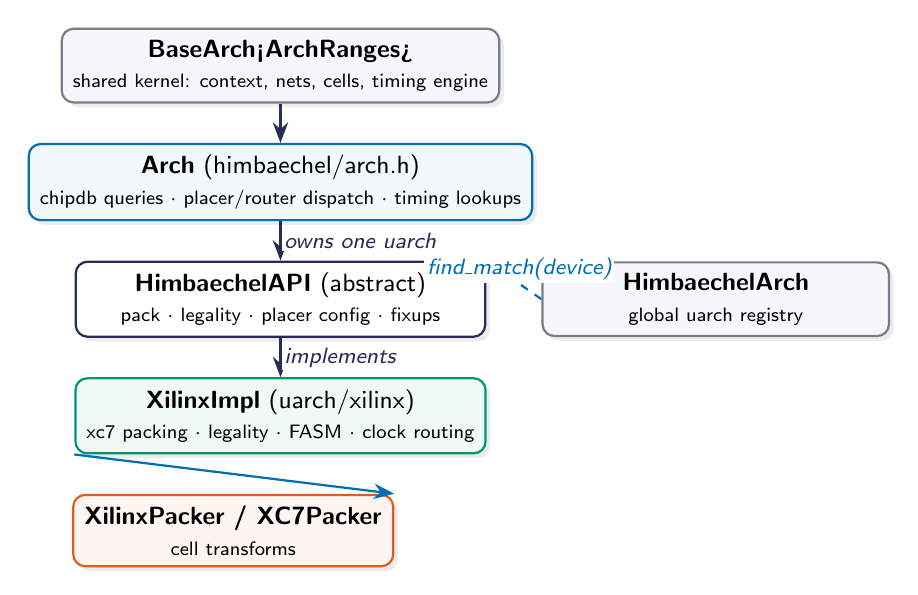
\begin{tikzpicture}[node distance=5mm]
  \node[flowboxgray, minimum width=52mm] (base) {\textbf{BaseArch<ArchRanges>}\\{\scriptsize shared kernel: context, nets, cells, timing engine}};
  \node[flowboxaccent, minimum width=52mm, below=of base] (arch) {\textbf{Arch} (himbaechel/arch.h)\\{\scriptsize chipdb queries $\cdot$ placer/router dispatch $\cdot$ timing lookups}};
  \node[flowbox, minimum width=52mm, below=of arch] (api) {\textbf{HimbaechelAPI} (abstract)\\{\scriptsize pack $\cdot$ legality $\cdot$ placer config $\cdot$ fixups}};
  \node[flowboxgreen, minimum width=52mm, below=of api] (xil) {\textbf{XilinxImpl} (uarch/xilinx)\\{\scriptsize xc7 packing $\cdot$ legality $\cdot$ FASM $\cdot$ clock routing}};
  \node[flowboxwarm, minimum width=40mm, below=5mm of xil, xshift=-6mm] (packer) {\textbf{XilinxPacker / XC7Packer}\\{\scriptsize cell transforms}};
  \node[flowboxgray, minimum width=44mm, right=7mm of api] (reg) {\textbf{HimbaechelArch}\\{\scriptsize global uarch registry}};
  \draw[arrdark] (base) -- (arch);
  \draw[arrdark] (arch) -- node[lbl,right] {owns one uarch} (api);
  \draw[arrdark] (api) -- node[lbl,right] {implements} (xil);
  \draw[arr] (xil.south west) -- (packer.north east);
  \draw[arr, dashed] (reg.west) -- node[lbl,above,pos=0.4] {find\_match(device)} (api.north east);
\end{tikzpicture}
\caption{Class structure: the generic Arch wraps exactly one uarch
plugin. At startup \texttt{Arch::Arch()} asks the global
\texttt{HimbaechelArch} registry which uarch matches the requested device
(\texttt{arch.cc:43-58}); for \texttt{xc7*} that is \texttt{XilinxImpl}.}
\label{fig:classes}
\end{figure}

The \texttt{HimbaechelAPI} interface is the contract every uarch must
fulfil. The important hook groups:

\begin{center}
\small\sffamily
\begin{tabularx}{\textwidth}{>{\bfseries\color{accent1}}l X}
\toprule
Hook & Responsibility \\
\midrule
\texttt{init\_database()} & validate/configure the chipdb, set speed grade, seed tags \\
\texttt{getUArchOptions()} & register family CLI options (e.g.\ \texttt{--fasm}, \texttt{--xdc}) \\
\texttt{pack()} & transform the logical netlist into physical cells (bels) \\
\texttt{prePlace /\newline postPlace} & tags, control-set indexing / post-placement fixups \\
\texttt{configurePlacerHeap /\newline configurePlacerStatic} & feed family parameters into the shared placers \\
\texttt{checkBelAvail /\newline checkPipAvail} & hard block resources (e.g.\ reserved pips) \\
\texttt{isBelLocationValid} & \emph{legality}: can this set of cells share this site? \\
\texttt{preRoute /\newline postRoute} & source/sink setup, clock routing / routing fixups, FASM \\
\texttt{getCellDelay /\newline lookupCellSeqTimings} & timing arcs for the shared timing engine \\
\bottomrule
\end{tabularx}
\end{center}

The Xilinx uarch exposes exactly two CLI options of its own:

\begin{cppfile}{himbaechel/uarch/xilinx/xilinx.cc:66}
  \lstinputlisting[style=cppstyle]{snippets/uarch_options.cc}
\end{cppfile}

% ===========================================================================
\section{The Xilinx uarch: packing}

Packing rewrites the technology-mapped netlist (LUTs, FFs, CARRY4s,
BRAMs, IOBs, \dots) into \emph{physical} cells that correspond 1:1 to
chipdb bels. The xc7 implementation is spread over
\texttt{himbaechel/\allowbreak uarch/\allowbreak xilinx/\allowbreak pack*.cc}; the top-level order is:

\begin{cppfile}{himbaechel/uarch/xilinx/pack.cc:821}
  \lstinputlisting[style=cppstyle]{snippets/pack_order.cc}
\end{cppfile}

Physical cell \emph{templates} are built in \texttt{cells.cc}; for
example every 6-LUT becomes a \texttt{SLICE\_LUTX} with the full A1--A6
/ WA1--WA8 port set (the WA ports exist so the same bel can serve as
distributed RAM):

\begin{cppfile}{himbaechel/uarch/xilinx/cells.cc:34}
  \lstinputlisting[style=cppstyle]{snippets/create_cell.cc}
\end{cppfile}

\begin{table}[htbp]
\centering
\small\sffamily
\begin{tabularx}{\textwidth}{>{\bfseries\color{accent1}\raggedright\arraybackslash}p{40mm} X >{\raggedright\arraybackslash}p{34mm}}
\toprule
Primitive family & Packed to & Packer (uarch/xilinx) \\
\midrule
LUT1--6, LUT6\_2 & \texttt{SLICE\_LUTX} (O5/O6) & \texttt{pack.cc} (pack\_luts) \\
FFs (FDRE/FDSE/$\dots$), latches & \texttt{SLICE\_FFX} & \texttt{pack.cc} (pack\_ffs) \\
MUXF7 / MUXF8 & \texttt{SELMUX2\_1} trees & \texttt{pack.cc} (pack\_muxfs) \\
CARRY4 & \texttt{MUXCY}/\texttt{XORCY} reassembled chains & \texttt{pack\_carry.cc} \\
SRL16E / SRLC32E & \texttt{SLICE\_LUTX} (SRL mode) & \texttt{pack.cc} (pack\_srls) \\
Distributed RAM (RAM64$\times$1S/D, RAM32M/64M, 128/256$\times$1S/D) & SLICEM LUTs + F7/F8 decode trees & \texttt{pack\_dram.cc} \\
Block RAM (RAMB18E1 / RAMB36E1, TDP+SDP) & \texttt{RAMB18E1}/\texttt{RAMB36E1} bels & \texttt{pack.cc} (pack\_bram) \\
DSP48E1 (+ cascades) & \texttt{DSP48E1\_DSP48E1} & \texttt{pack\_dsp\_xc7.cc} \\
IO buffers, IDDR/ODDR, ISERDESE2/OSERDESE2, IDELAYE2/ODELAYE2, IDELAYCTRL & IOB33 (HR) / IOB18 (HP) + IOLOGIC & \texttt{pack\_io.cc} \\
BUFG/BUFGCE/BUFGCTRL, MMCME2, PLLE2, BUFR/BUFIO/BUFHCE & clocking sites & \texttt{pack\_clocking.cc} \\
PS7 (Zynq) & \texttt{PS7\_PS7} & \texttt{pack\_io.cc} \\
\bottomrule
\end{tabularx}
\caption{Primitive coverage of the xc7 uarch in this checkout (full
matrix, with limitations, in the porting analysis).}
\end{table}

% ===========================================================================
\section{Placement: shared algorithms, family legality}

\subsection{Dispatch}

The generic Arch dispatches to one of three shared placers selected by
\texttt{--placer}; the Xilinx uarch defaults to \texttt{heap} and maps
its default router to \texttt{router2} (\texttt{xilinx.h:147}):

\begin{cppfile}{himbaechel/arch.cc:266}
  \lstinputlisting[style=cppstyle]{snippets/place_dispatch.cc}
\end{cppfile}

\subsection{HeAP: the analytical placer}

\texttt{placer\_heap} (``HeAP'') is the default. Each iteration:

\begin{enumerate}
\item \textbf{Bind constraints}---every \texttt{BEL}-attributed cell is
  placed with \texttt{STRENGTH\_USER}.
\item \textbf{Solve}---cells are modelled as bound-to-bound springs; an
  Eigen Conjugate-Gradient solve produces x/y positions for each bel
  bucket run.
\item \textbf{Spread}---\texttt{CutSpreader} pushes overlapping cells
  apart per cell group, respecting group areas.
\item \textbf{Legalise}---\texttt{StrictLegaliser} walks cells to legal
  sites (a greedy random-walk with bel buckets and control-set
  pre-allocation), checking uarch legality on every candidate.
\item \textbf{Timing}---a timing pass if \texttt{timing\_driven}.
\end{enumerate}

The loop keeps the best snapshot, then finishes with a refinement pass
(\texttt{parallel\_refine} or \texttt{placer1\_refine}). The
alternatives are \texttt{placer\_static} (ePlace-style electrostatic
placement via FFT density solves with Nesterov acceleration---good for
large designs) and \texttt{placer1} (classic simulated annealing).

\subsection{What the Xilinx uarch configures}

The uarch teaches the placer about xc7 structure via
\texttt{configurePlacerHeap}:

\begin{cppfile}{himbaechel/uarch/xilinx/xilinx.cc:321}
  \lstinputlisting[style=cppstyle]{snippets/configure_placerheap.cc}
\end{cppfile}

Two ideas matter here. \textbf{Clusters}: related physical cells (a
CARRY4 and its LUTs, an F7MUX tree, a DRAM decode tree) are grouped as
\texttt{ClusterId}s; the placer moves clusters atomically and asks the
uarch for each member's offset via \texttt{getClusterPlacement}
(\texttt{arch.h:744-756}). \textbf{Control sets}: xc7 FFs in one half
slice must share CLK/SR/CE (and their inversion bits), so the uarch
pre-indexes control sets (\texttt{index\_control\_sets},
\texttt{xilinx.cc:617-635}) and hands the placer
\texttt{ff\_control\_set\_groups} plus a radius ladder
(\texttt{ctrl\_set\_max\_radius} $\{18,15,12,9,6,3\}$) to keep
same-control-set FFs near each other.

\subsection{Legality: the heart of xc7 placement}

The placer is family-agnostic; the uarch decides whether a set of cells
may legally share a site. For logic tiles that is
\texttt{XilinxImpl::xc7\_logic\_tile\_valid} (\texttt{xilinx\_place.cc:43}),
fed by per-tile \texttt{LogicTileStatus} caches that track which cells
occupy which bel:

\begin{cppfile}{himbaechel/uarch/xilinx/xilinx_place.cc:43}
  \lstinputlisting[style=cppstyle]{snippets/logic_tile_valid.cc}
\end{cppfile}

The checker enforces, per eight (four LUT/FF columns) and per half
slice:

\begin{itemize}
\item \textbf{SLICEM/SLICEL rules}---memory and SRL LUTs only in SLICEM
  (the ``M'' tiles), SRLs only in the bottom half;
\item \textbf{5LUT coexistence}---a 5LUT may not sit under a 6-input or
  dual-output 6LUT; combined inputs must overlap sufficiently;
\item \textbf{the X-input budget}---the F7MUX/F8MUX selects, the CARRY4
  x-sigs, and any indirect FF D inputs must all agree on a single X net
  per position;
\item \textbf{output-mux exclusivity}---O5, F7F8, carry-out and FF2
  cannot all demand the single output mux;
\item \textbf{half-tile control sets}---CLK/SR/CE plus their inversion,
  latch and sync bits must match across all eight FFs, and the
  distributed-RAM write clock must equal the FF clock in the bottom
  half.
\end{itemize}

\begin{warnbox}{Known gap in this checkout}
The analysis in \texttt{../xilinx-porting/03-algorithmic-diff.md} shows
this checker still lacks several legality rules the openXC7 fork had to
add over years of silicon debugging: the per-position site-exit
(OUTMUX) budget, cross-position carry$\to$FF pairing rejection,
FF1-via-X + 5FF co-pack rejection, and SRL cascade placement. Porting
those checks is work package WP1 of the porting plan---without them the
legaliser can silently produce illegal slices.
\end{warnbox}

After placement, \texttt{fixup\_placement}
(\texttt{xilinx\_place.cc:389}) re-permutes LUT5/LUT6 inputs onto
non-overlapping A pins and records the logical mapping in
\texttt{X\_ORIG\_PORT\_*} attributes---the bridge between nextpnr's
free LUT input ordering and RapidWright/Vivado's fixed physical
ordering.

% ===========================================================================
\section{Routing: router2 and the Xilinx glue}

Routing uses the shared \texttt{router2} (default) or \texttt{router1}.
Router2 is a bidirectional meet-in-the-middle A* search:

\begin{figure}[htbp]
\centering
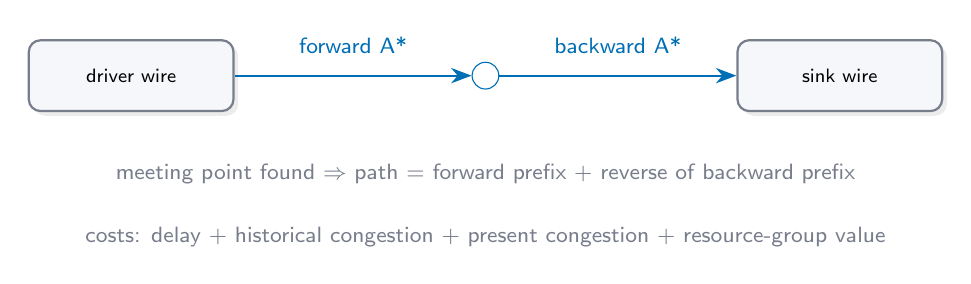
\begin{tikzpicture}
  \node[flowboxgray, minimum width=26mm] (src) at (0,0) {\scriptsize driver wire};
  \node[flowboxgray, minimum width=26mm] (dst) at (9,0) {\scriptsize sink wire};
  \node[draw=accent1, circle, inner sep=1.2mm] (m) at (4.5,0) {};
  \draw[arr, accent1] (src.east) -- node[above=1.5mm, font=\sffamily\footnotesize, color=accent1] {forward A*} (m.west);
  \draw[arr, accent1] (m.east) -- node[above=1.5mm, font=\sffamily\footnotesize, color=accent1] {backward A*} (dst.west);
  \node[font=\sffamily\footnotesize\color{grayline}, anchor=north] at (4.5,-1.0)
       {meeting point found $\Rightarrow$ path = forward prefix + reverse of backward prefix};
  \node[font=\sffamily\footnotesize\color{grayline}, anchor=north] at (4.5,-1.8)
       {costs: delay + historical congestion + present congestion + resource-group value};
\end{tikzpicture}
\caption{Router2 searches from both ends of each arc and stitches the
two halves at a meeting wire. Congestion is tracked per wire and per
\emph{resource group} (the uarch's \texttt{getResourceKeyForPip}), and
the routing is checked by a router1 pass at the end.}
\label{fig:router2}
\end{figure}

The Xilinx uarch adds family-specific routing phases around the shared
core (\texttt{preRoute}/\texttt{postRoute} in \texttt{xilinx.cc}):

\begin{itemize}
\item \texttt{find\_source\_sink\_locs()}---precomputes the source and
  sink locations for each net for the router;
\item \texttt{route\_clocks()} (\texttt{pack\_clocking.cc})---routes
  the dedicated clock backbone (BUFG$\to$HROW\allowbreak$\to$CK\_MUXED) before
  general routing so ordinary signals cannot claim clock resources;
\item \texttt{fixup\_routing()} (\texttt{xilinx\_place.cc:512})---after
  routing, converts any LUT-permutation pips the router used into
  physical connections and records the permutation in
  \texttt{X\_ORIG\_PORT\_*} (again for RapidWright compatibility), and
  legalises OSERDESE3 bypasses.
\end{itemize}

\subsection{Delay estimation}

The router's cost function needs wire and pip delays. Himbaechel
computes them from the chipdb timing classes (see \S\ref{sec:timing});
the Xilinx uarch overrides \texttt{estimateDelay}/\texttt{predictDelay}
(\texttt{xilinx.cc:735-780}) with heuristics that the source itself
marks as improvable (\texttt{TODO: improve sophistication here based on
old nextpnr-xilinx code}).

% ===========================================================================
\section{Timing}
\label{sec:timing}

Timing data is baked into the chipdb as three POD families:

\begin{itemize}
\item \textbf{Pip timing}---per pip class: intrinsic delay, input
  capacitance, output resistance;
\item \textbf{Node timing}---capacitance/resistance/delay for merged
  cross-tile nodes;
\item \textbf{Cell timing}---per cell type: combinational arcs and
  sequential arcs (setup/hold/clock-to-Q).
\end{itemize}

At run time the generic Arch implements the shared timing-engine
callbacks (\texttt{getCellDelay}, \texttt{getPortTimingClass},
\allowbreak\texttt{getPortClockingInfo}) by looking these PODs up
(\texttt{arch.cc:470-520}); the Xilinx uarch only supplies the
family-specific details---for instance BRAM timing variants (write-TDP
vs.\ write-SDP $\times$ read-TDP vs.\ read-SDP) are selected by
rewriting the cell's timing index (\texttt{xilinx.cc:602-612}).

Clock constraints flow through two stages: \texttt{create\_clock}
periods from the XDC parser land on nets (\texttt{xdc.cc}), and
\texttt{generate\_constraints} (\texttt{pack\_clocking.cc:384-535})
propagates them through BUFGCTRL/IBUF/PLL/MMCM, computing VCO and
output-clock frequencies so downstream logic is analysed against
derived clocks.

\begin{warnbox}{Timing limitations in this checkout}
Only one speed grade (\texttt{DEFAULT}) is generated
(\texttt{gen/xilinx\_gen.py:387}), and LUT/FF timing is stubbed rather
than imported from SDF (\texttt{gen/xilinx\_gen.py:450-462})---so
timing-driven flows currently lean on BRAM/SELMUX2\_1/CARRY4 arcs plus
heuristics. This is a known limitation tracked in the porting analysis.
\end{warnbox}

% ===========================================================================
\section{FASM: from routed design to bitstream}

The final stage writes an \emph{abstract bitstream} in FASM (FPGA
Assembly) format---one human-readable line per configured feature:

\begin{figure}[htbp]
\centering
\resizebox{\textwidth}{!}{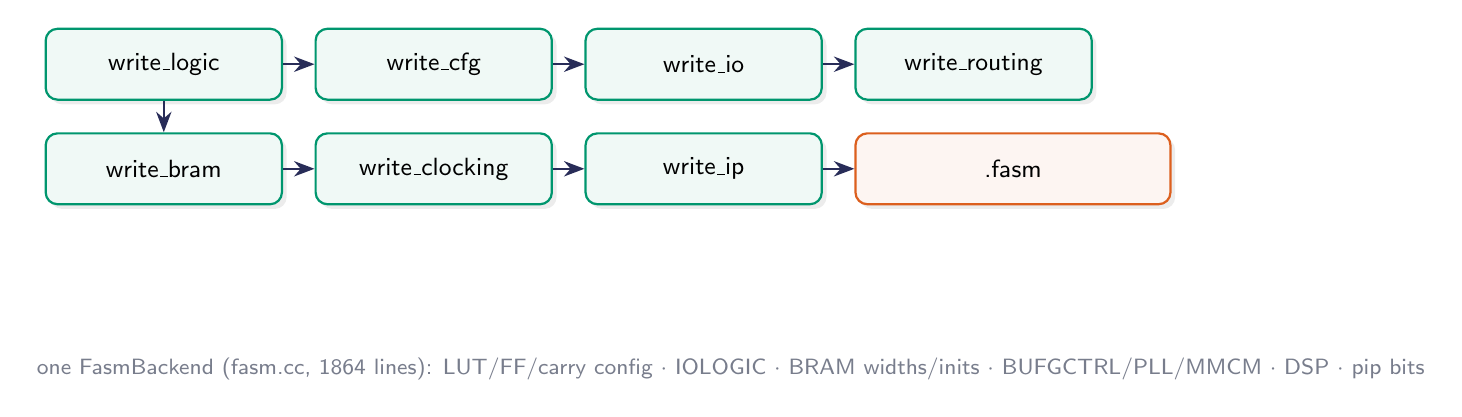
\begin{tikzpicture}[node distance=4mm]
  \node[flowboxgreen, minimum width=30mm] (l) {write\_logic};
  \node[flowboxgreen, minimum width=30mm, right=of l] (c) {write\_cfg};
  \node[flowboxgreen, minimum width=30mm, right=of c] (io) {write\_io};
  \node[flowboxgreen, minimum width=30mm, right=of io] (r) {write\_routing};
  \node[flowboxgreen, minimum width=30mm, below=of l] (b) {write\_bram};
  \node[flowboxgreen, minimum width=30mm, right=of b] (k) {write\_clocking};
  \node[flowboxgreen, minimum width=30mm, right=of k] (ip) {write\_ip};
  \node[flowboxwarm, minimum width=40mm, right=of ip] (out) {.fasm};
  \draw[arrdark] (l) -- (c);
  \draw[arrdark] (c) -- (io);
  \draw[arrdark] (io) -- (r);
  \draw[arrdark] (l) -- (b);
  \draw[arrdark] (b) -- (k);
  \draw[arrdark] (k) -- (ip);
  \draw[arrdark] (ip) -- (out);
  \node[font=\sffamily\footnotesize\color{grayline}, anchor=north] at (7.2,-3.6)
       {one FasmBackend (fasm.cc, 1864 lines): LUT/FF/carry config $\cdot$ IOLOGIC $\cdot$ BRAM widths/inits $\cdot$ BUFGCTRL/PLL/MMCM $\cdot$ DSP $\cdot$ pip bits};
\end{tikzpicture}}
\caption{The FASM writer walks the routed design section by section and
emits feature lines. External prjxray tools (\texttt{fasm2frames},
\texttt{xc7frames2bit}, via \texttt{examples/\allowbreak bitgen\_xray.sh}) then
assemble the physical bitstream.}
\label{fig:fasm}
\end{figure}

FASM keeps the last step independent of Vivado: the features reference
prjxray-documented bit positions, so the whole xc7 flow (Yosys
$\to$ nextpnr $\to$ fasm2frames $\to$ xc7frames2bit) is
fully open source. Pseudo-pips (config-only pips with no real
connection) are handled by a \texttt{(tileType,dest,source)} table in
the FASM backend, and LUT input permutations are re-encoded as
\texttt{X\_ORIG\_PORT} attributes rather than emitted as pip bits.

% ===========================================================================
\section{Device support today}

\begin{table}[htbp]
\centering
\small\sffamily
\begin{tabular}{>{\bfseries\color{accent1}}l l l}
\toprule
Family & Site metadata (meta/) & Devices in default build \\
\midrule
artix7 & SLICEL/M, IOB33, GTPE2, PCIE\_2\_1, $\dots$ & xc7a50t, xc7a100t, xc7a200t (+ a35t alias) \\
kintex7 & IOB18/33, GTXE2, ODELAYE2, $\dots$ & --- (code path exists, not in default list) \\
spartan7 & IOB33, ILOGICE3/OLOGICE3, $\dots$ & xc7s50 \\
zynq7 & + PS7, IOB18/33 & xc7z010, xc7z020 \\
\bottomrule
\end{tabular}
\caption{Device coverage in this checkout. Kintex-7 metadata exists but
no xc7k device is enabled by default---a one-line CMake change (see the
porting plan WP0).}
\end{table}

UltraScale(+) is \emph{not} served by this uarch: \texttt{match\_device}
accepts only \texttt{xc7*} (\texttt{xilinx.cc:815}). The separate
\texttt{ng-ultra} uarch targets a different UltraScale-class part
(``Project Beyond''), and the E2/E3-era identifiers in the shared
\texttt{constids.inc} are a superset vocabulary without packers. Porting
the openXC7 fork's UltraScale+ (xcup) flow is its own work package.

% ===========================================================================
\appendix
\section{Glossary}

\begin{description}[style=nextline, font=\sffamily\bfseries\color{accent1}, itemsep=3pt]
\item[chipdb] The compile-time-generated, position-independent binary
  device database, memory-mapped at run time.
\item[bel] Basic Element of Logic---one atomic site resource (a LUT, a
  FF, a BRAM, a pad); ``bel'' in nextpnr.
\item[pip] Programmable Interconnect Point---one configurable switch
  between two wires (or between a site wire and a bel pin).
\item[node] A merged group of electrically-connected tile wires; the
  unit of net identity across tile boundaries.
\item[uarch] A himbaechel micro-architecture plugin (one
  \texttt{HimbaechelAPI} subclass) for a device family.
\item[RelPtr / RelSlice] Relative pointer / relative slice---offset-based
  references that make the chipdb position-independent.
\item[FASM] FPGA Assembly---the textual feature-per-line interchange
  format emitted by nextpnr and consumed by prjxray tools.
\item[X\_ORIG\_PORT] Attribute recording the original logical LUT input
  ordering after nextpnr permutes physical inputs; keeps
  RapidWright/Vivado-compatible names.
\end{description}

\section{Where the details live}

\begin{itemize}
\item Architecture analysis, feature inventory, algorithmic diff and the
  porting plan: \texttt{docs/\allowbreak xilinx-porting/} in this repository.
\item Upstream framework documentation: \texttt{docs/himbaechel.md}.
\item Chipdb POD definitions: \texttt{himbaechel/chipdb.h}.
\item Xilinx uarch implementation: \texttt{himbaechel/uarch/xilinx/}.
\item Shared placers/routers: \texttt{common/place/},
  \texttt{common/route/}.
\end{itemize}

\end{document}
